\documentclass[10pt,twocolumn]{article}

\usepackage{bold-extra}
\usepackage{color}
\usepackage{float}
\usepackage{graphicx}
\usepackage{listings}
\usepackage{subfigure}
\usepackage{url}

%%%%%%%%%%%%%%%
%%% Colours %%%
%%%%%%%%%%%%%%%

\definecolor{darkgreen}{rgb}{0, 0.6, 0}
\definecolor{lightgrey}{gray}{0.9}

%%%%%%%%%%%
% Figures %
%%%%%%%%%%%

\newcommand{\stufigex}[5]					% images with specified placement
{
	\begin{figure}[#5]
	\begin{center}
		\includegraphics[#1]{#2}
		\caption{#3}
		\label{#4}
	\end{center}
	\end{figure}
}

% Define the stusubfig environment
\newenvironment{stusubfig}[1]
{
	\begin{figure*}[#1]
	\begin{center}
}
{
	\end{center}
	\end{figure*}
}

%%%%%%%%%%%%%%%%%
% Code Listings %
%%%%%%%%%%%%%%%%%

% Create a new type of float (called a stulisting) for listings
\floatstyle{ruled}
\newfloat{stulisting}{thp}{lop}
\floatname{stulisting}{Listing}

% Setup before using the listings package
\renewcommand{\lstlistingname}{\textbf{Listing}}
\def\thelstlisting{\textbf{\arabic{lstlisting}}}

\lstdefinelanguage{Pseudocode}{
morekeywords={and,assert,break,case,continue,default,down,each,else,for,function,if,not,null,or,rangeswitch,ref,return,switch,then,this,throw,to,up,var,while},
sensitive=true,
morecomment=[l]{//},
morecomment=[s]{/*}{*/}
}

\lstdefinestyle{Default}{
abovecaptionskip=0.5cm,
basicstyle=\scriptsize\ttfamily,
belowcaptionskip=0.5cm,
belowskip=0.5cm,
columns=fixed,
%commentstyle=\color{darkgreen},
commentstyle=\textit, % changed from the thesis (green text looks unprofessional in a journal paper)
language=Pseudocode,
%numbers=left,
numbers=none, % changed from the thesis (line numbers are less relevant here)
numbersep=5pt,
numberstyle=\tiny,
mathescape=true,
showstringspaces=false,
stepnumber=1,
tabsize=4
}

\lstdefinestyle{Snippet}{
abovecaptionskip=0.5cm,
aboveskip=0.5cm,
basicstyle=\small\ttfamily,
belowcaptionskip=0.5cm,
belowskip=0.5cm,
columns=fixed,
commentstyle=\color{darkgreen},
frame=lines,
keywordstyle=\small\bfseries,
language=Pseudocode,
numbers=none,
mathescape=true,
showstringspaces=false,
stepnumber=1,
tabsize=4
}

% For C++ function prototypes
\lstdefinestyle{Prototype}{
abovecaptionskip=0.5cm,
basicstyle=\small\ttfamily,
belowcaptionskip=0.5cm,
belowskip=0.5cm,
columns=fixed,
commentstyle=\color{darkgreen},
language=C++,
numbers=none,
mathescape=true,
showstringspaces=false,
stepnumber=1,
tabsize=4
}

%%%%%%%%%%%%%%%%%
% Main Document %
%%%%%%%%%%%%%%%%%

\begin{document}

\title{Implementing Automatic Navigation Mesh Generation in Configuration Space}
\author{Stuart Golodetz}
\date{}
\maketitle

\section{Introduction}

The representation of the walkable area of a 3D environment in such a way as to facilitate successful navigation by intelligent agents is an important problem in the computer games and artificial intelligence fields, and it has been extensively studied. As surveyed by Tozour \cite{tozour04}, there are a variety of common ways to represent such an environment, including regular grids, which support random-access lookup but do not translate easily into a 3D context, use a lot of memory and can yield aesthetically unpleasing paths; waypoint graphs -- connecting large numbers of nodes (often manually placed) with edges that imply walkability in the game world -- these were previously popular in games but are costly to build and tend to constrain agents to walking `on rails' between connected waypoints; space-filling volumes, which entail growing randomly-placed seeds to try and fill the free space in the level; and navigation meshes, that represent the walkable surface of a world explicitly using a polygonal mesh. Polygons within a navigation mesh are connected using links that imply the ability of the agent to walk/step/jump/etc.\ between them (see Figure~\ref{fig:navmeshexample}).

%---
\stufigex{width=.9\linewidth}{blakeney-upperramp-clearer.png}{An example navigation mesh and its links: cyan = walk link; magenta = step up link; yellow = step down link.}{fig:navmeshexample}{t}
%---

Since their introduction by Greg Snook \cite{snook00}, navigation meshes have proved to be a particularly successful approach due to their ability to represent the free space available around paths through the world (this is extremely useful because it provides the pathfinder with the information it needs to successfully avoid local obstacles). As a result, they have seen widespread use in both games themselves, and popular games engines such as Source and Unreal, and many games authors have contributed to their theoretical development (most notably in the \emph{Game Programming Gems} and \emph{AI Game Programming Wisdom} book series). There has also been significant interest from researchers in academia (e.g.~see \cite{hale09,kallmann10,pettre05,vantoll11}).

%---
\begin{stusubfig}{!t}
	\subfigure[Finding the intersection of a half-ray through the nearest vertex of the AABB with the plane]
	{\hspace{6mm}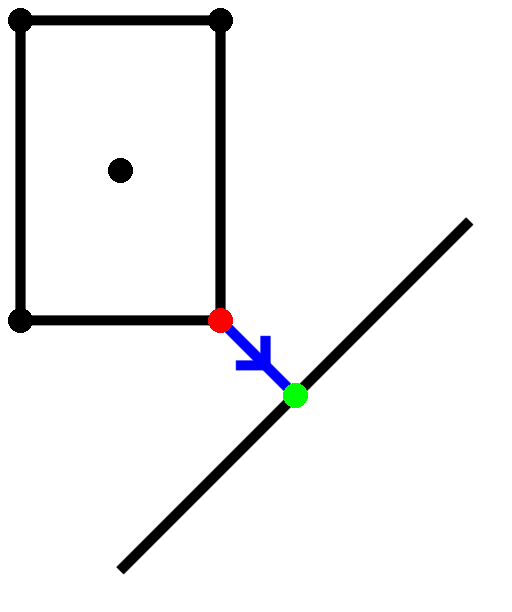
\includegraphics[width=.2\linewidth]{aabbvsplane-a.png}\hspace{6mm}}%
	%
	\hspace{10mm}%
	%
	\subfigure[Expanding the plane to form a configuration space]
	{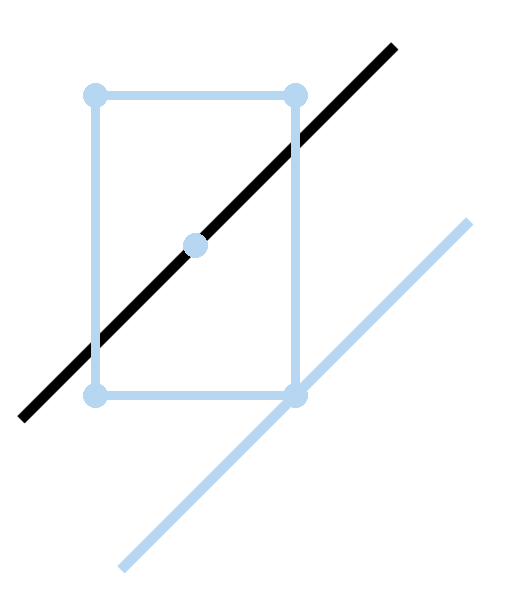
\includegraphics[width=.2\linewidth]{aabbvsplane-b.png}}%
	%
	\hspace{10mm}%
	%
	\subfigure[Finding the intersection of a half-ray through the centre of the AABB with the expanded plane]
	{\hspace{6mm}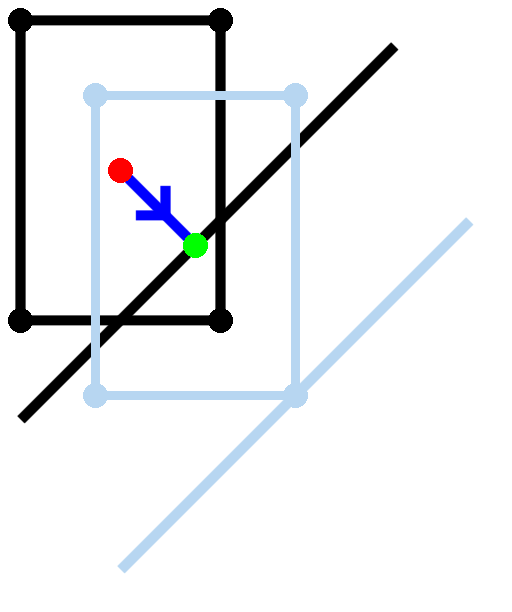
\includegraphics[width=.2\linewidth]{aabbvsplane-c.png}\hspace{6mm}}%
\caption{Detecting the first collision point between a translating AABB and a plane.}
\label{fig:aabbvsplane}
\end{stusubfig}
%---

One facet of using navigation meshes is how to build them in the first place, and numerous methods have been described in the literature, of which a few examples are described here. An early approach due to Tozour \cite{tozour02} works by first determining the walkable polygons in a 3D environment by comparing their normals with the up vector, and then iteratively merging together as many polygons as possible using the Hertel-Mehlhorn algorithm \cite{hertel83,orourke94} and a $3 \rightarrow 2$ merging technique. Hamm \cite{hamm08} generates a navigation mesh using an empirical method that involves sampling the environment to create a grid of points, identifying a subset of points both on the boundary of and within the environment, and connecting these points to form a mesh. Ratcliff \cite{ratcliff08} creates a navigation mesh by tessellating all walkable surfaces in the world, merging the results together to form suitable nodes and then computing links between neighbouring nodes. Van Toll \emph{et al.} \cite{vantoll11} build a navigation mesh for a multi-layer environment by constructing a mesh based on the medial axis for each layer and then connecting the medial axes by `opening' the connections between the layers. The same authors later demonstrated how such a mesh could be dynamically modified \cite{vantoll12}. Mononen's open-source Recast library \cite{mononen09} first voxelizes the 3D environment before running a watershed transform \cite{beucher90,gonzalez02} on the walkable voxels and creating a mesh from the resulting partition of the walkable surface.

%TODO: Survey the various methods \cite{axelrod08,farnstrom06,hale11,kallmann10,mcanlis08,mononen09,oliva11,pettre05,ratcliff08,vanwaveren01,wein05}.

In this article, I describe the implementation of navigation mesh construction in my homemade \emph{hesperus} engine \cite{hesperus}, based heavily on the approach of van Waveren in \cite{vanwaveren01}. The goal is to provide a helpful, implementation-focused introduction for those with no prior experience in the area. At a high-level, the method is as follows:
%
\begin{enumerate}
\item Given a 3D environment made up of brushes (simple convex polyhedra, each consisting of a set of polygonal faces), and a set of axis-aligned bounding boxes (AABBs) used to represent the possible sizes of the agents that will navigate the environment, expand the brushes by appropriate amounts (see \S\ref{sec:configspace}) to create a set of expanded brushes for each AABB.
\item Using constructive solid geometry (CSG) techniques, union the expanded brushes for each AABB together to form a polygonal environment. Filter the polygons of the environment to find those that are \emph{walkable} (judged by comparing their face normals with the up vector). This gives us the polygons of a navigation mesh for each AABB, but without any links to indicate how agents should navigate between them. See \S\ref{sec:meshgen}.
\item Generate walk and step links between the polygons of each navigation mesh (see \S\ref{sec:walkstep}) -- these indicate, respectively, that an agent can walk from one polygon of the mesh to another, or step up/down from one polygon to another. These links can be used to generate a graph for the purposes of path planning.
\end{enumerate}
%
The following sections look at each of these steps in more detail.

\section{Configuration Spaces}
\label{sec:configspace}

%---
\begin{stusubfig}{!t}
	\subfigure[A brush-based environment]
	{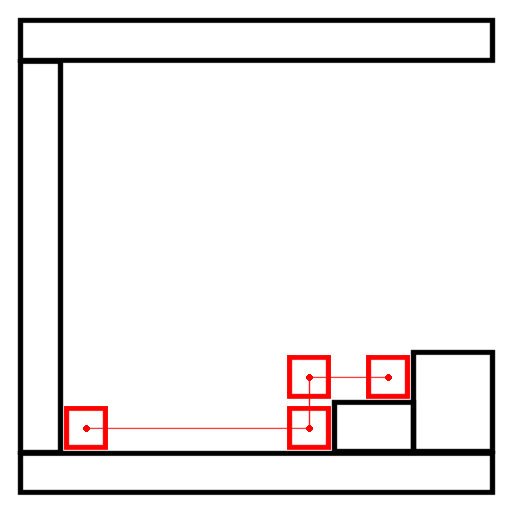
\includegraphics[width=.3\linewidth]{configspace-before.png}}%
	%
	\hspace{4mm}%
	%
	\subfigure[Configuration space]
	{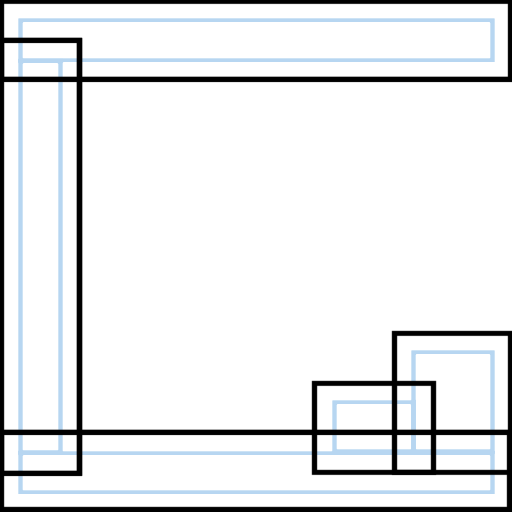
\includegraphics[width=.3\linewidth]{configspace-after.png}}%
	%
	\hspace{4mm}%
	%
	\subfigure[A bevel plane]
	{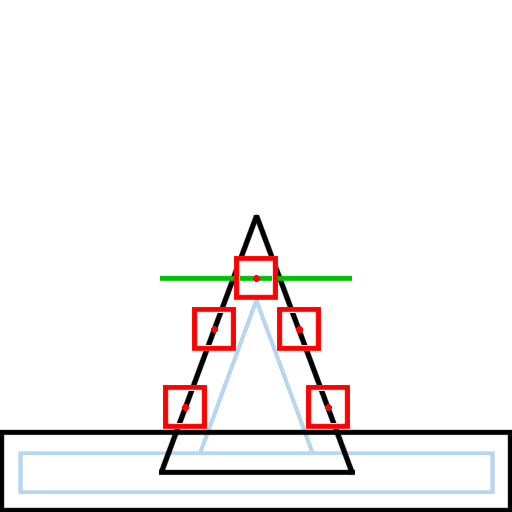
\includegraphics[width=.3\linewidth]{configspace-bevel.png}}%
\caption{A configuration space can be generated for the entirety of a brush-based environment by expanding all of the brushes by an appropriate amount: (a) shows a brush-based environment, together with the range of movement of a simple agent; (b) shows the configuration space that would be generated for that agent; (c) shows that expanding non-axis-aligned brushes may require \emph{bevel} planes (shown in green) in order to correctly determine the range of movement.}
\label{fig:configspace}
\end{stusubfig}
%---

When planning the movement of intelligent agents (e.g.~robots), a \emph{configuration space} is the space of possible configurations in which an agent can validly exist. As a first example of what this concept means and when it can be useful, consider detecting the first point of collision between a plane and an AABB that is moving by translation only -- this might normally involve determining which vertex of the AABB is nearest to the plane and finding the point at which a half-ray oriented in the AABB's direction of movement and starting at that vertex would intersect the plane (see Figure~\ref{fig:aabbvsplane}(a)). The configuration space alternative is to initially expand the plane in the direction of its normal by a fixed amount so that the centre of the AABB touches the expanded plane precisely when the nearest vertex of the AABB touches the non-expanded plane (see Figure~\ref{fig:aabbvsplane}(b)). The first point of intersection can then be calculated by finding the point at which a half-ray starting at the centre of the AABB would touch the expanded plane (see Figure~\ref{fig:aabbvsplane}(c)) -- there is no longer a need to first determine which vertex is nearest to the plane. Put another way: by expanding the plane, we have created the space of possible configurations for the centre of the AABB, and thereby restricted our testing to making sure that the AABB's centre is always in a valid location.

As explained in \cite{vanwaveren01}, the concept of configuration space can be extended to an entire 3D environment, allowing us to test an agent represented as an AABB against such an environment using only point-based (rather than AABB-based) intersection tests: this was the approach taken in the popular \emph{Quake III Arena} game. Starting with a \emph{brush-based} 3D environment (i.e.~one that is built up by combining instances of simple convex polyhedra such as cuboids, cylinders and cones -- a common approach in 3D world editors), a configuration space for agents with a specific AABB can be constructed by expanding each brush by an appropriate amount (see Figure~\ref{fig:configspace}(a) and (b)). Note that expanding each brush correctly can require the introduction of additional \emph{bevel} planes as described in \cite{vanwaveren01} (see Figure~\ref{fig:configspace}(c)).

\section{Basic Mesh Generation}
\label{sec:meshgen}

\subsection{Brush Unioning}

Having expanded the brushes of a brush-based environment to construct a configuration space for an AABB in the manner described, the next step is to union the expanded brushes together to generate a set of polygons that represent the expanded environment as a whole. These polygons can then be processed further to construct a navigation mesh.

In conceptual terms, the process of brush unioning is relatively simple: given an input set of brushes, each of which consists of a set of (outward-facing) polygonal faces, it suffices to clip each brush face to all the other brushes within range of its own brush in the environment (see Figure~\ref{?}). From an implementation perspective, a convenient way to do this is to build a binary space partitioning (BSP) tree for each brush and clip each face to the trees of the other brushes. The high-level implementation of this process can be found in Listing~\ref{code:brush-unioning} and full source code is available online \cite{hesperus}. The end result is a set of polygons that represent the expanded environment.

%---
\begin{stulisting}[t]
\caption{Brush Unioning}
\label{code:brush-unioning}
\lstinputlisting[style=Default]{brush-unioning.lst}
\end{stulisting}
%---

\subsection{Finding Walkable Polygons}

Given the set of polygons generated in the previous section, finding those polygons that are \emph{walkable} is straightforward: it suffices to compare the angle between each polygon's normal, $\mathbf{\hat{n}}$ and the up vector ($\mathbf{\hat{u}} = (0,0,1)^T$) to some predefined threshold. The angle can be computed using the dot product:
%
\[
\theta = \cos^{-1} \left( \mathbf{\hat{n}} \cdot \mathbf{\hat{u}} \right)
\]
%
We then keep precisely those polygons whose angle is less than or equal to the threshold. In the \emph{hesperus} engine, a suitable threshold for human characters was found to be $\pi/4$ (i.e.~45 degrees to the horizontal).

\section{Walk and Step Links}
\label{sec:walkstep}

To generate simple links between walkable polygons in a navigation mesh, the general strategy is as follows:
%
\begin{enumerate}
\item We first create an \emph{edge plane table} that maps each vertical plane through one or more walkable polygon edges to two sets of edges that lie in the plane (edges in one set are oriented in the same direction as a `canonical' plane; edges in the other have the opposite orientation).
\item For each plane in the table and for each pair of opposing edges for that plane, we check to see whether any links need to be created. This is done by projecting the opposing edges into the plane and calculating the intervals (if any) in which the various types of link need to be created.
\end{enumerate}

\subsection{Edge Plane Table Construction}

%---
\begin{stulisting}[t]
\caption{Edge Plane Table Construction}
\label{code:ept-construction}
\lstinputlisting[style=Default]{ept-construction.lst}
\end{stulisting}
%---

The edge plane table is a map of type $\mbox{Plane} \to (\{\mbox{Edge}\},\{\mbox{Edge}\})$. To construct it, we proceed as shown in Listing~\ref{code:ept-construction}. For each edge of a walkable polygon, we first build the vertical plane passing through it and then add it to the table based on its facing with regard to the `canonical' vertical plane through the edge. This has the effect of separating the edges of walkable polygons into two sets on each vertical plane that can then be checked against each other in a pairwise manner to create navigation links -- see Figure~\ref{?} for an example. A few details are needed to make this work:
%
\begin{enumerate}

\item \emph{Vertical Plane Construction}. The edge is necessarily non-vertical (because it belongs to a walkable polygon), so the normal vector of the vertical plane can be calculated straightforwardly using a cross-product. If the endpoints of the edge are $\mathbf{p_1}$ and $\mathbf{p_2}$, and $\mathbf{\hat{u}}$ is once again the up vector, then the desired normal can be calculated as:
%
\[
\mathbf{n} = (\mathbf{p_2} - \mathbf{p_1}) \times \mathbf{\hat{u}}
\]
%
Normalising this to give $\mathbf{\hat{n}} = \mathbf{n} / \left|\mathbf{n}\right|$, the equation of the desired plane is then:
%
\[
\mathbf{\hat{n}} \cdot \mathbf{x} = \mathbf{\hat{n}} \cdot \mathbf{p_1}
\]

\item \emph{Canonical Plane Determination}. Given a plane with equation $ax + by + cz - d = 0$, we define the `canonical' form of this plane to be the one where the first of $a$, $b$ or $c$ to be non-zero is positive. Thus, the canonical form of both $0x + 1y - 1z - 23 = 0$ and $0x - 1y + 1z + 23 = 0$ would be $0x + 1y - 1z - 23 = 0$. Note that a plane is either already in canonical form, or can be canonicalised straightforwardly by negating all of its coefficients.

\item \emph{Plane Ordering}. In order to use planes as the key for the edge plane table, we need to define a suitable way of ordering them. This can be done using a variant of the approach described in \cite{salesin92}. In practice, the ordering was found to be easier to debug (although somewhat less efficient) if implemented as shown in Listing~\ref{code:plane-ordering}.

\end{enumerate}

%---
\begin{stulisting}[t]
\caption{Plane Ordering}
\label{code:plane-ordering}
\lstinputlisting[style=Default]{plane-ordering.lst}
\end{stulisting}
%---

\subsection{Link Creation}

TODO

\section{Potential Extensions}

At present, only walk and step links are implemented in \emph{hesperus}, but there are various additional links that it would be helpful to add.

\subsection{Crouch Links}

One obvious extension is to add \emph{crouch} links -- these are links that tell agents when they need to crouch in order to traverse low areas (e.g.~a low archway or a pipe). As the example in Figure~\ref{fig:crouchlinks} illustrates, these are inter-mesh links; they should be created so as to link the standing and crouching meshes for an agent at the boundary of areas that can be traversed on the crouching mesh but not on the standing one. Assuming that the AABBs for the two meshes differ only in their heights (as is the case in the example), one way of automatically detecting crouch links would be to match edges on the standing mesh that do not cause any walk or step links to be created with edges in the same plane on the crouching mesh that do.

%---
\stufigex{width=.9\linewidth}{crouchlinks.png}{Creating crouch links between navigation meshes can allow tall characters to pass through low areas. Here, crouch links should be created between the standing (green) and crouching (red) meshes to allow agents to traverse this low archway.}{fig:crouchlinks}{t}
%---

\subsection{Ladder Links}

The addition of ladder links (indicating that an agent can travel from one floor to another using a ladder) is not conceptually very difficult, but it requires tool support. In \emph{hesperus}, the map editor would need to be augmented to handle ladders and other static entities; when placing a ladder, it would then be a simple matter to create a link at either end of the ladder to represent travel in each direction. It should be noted that \emph{traversing} ladder links is significantly more complicated than traversing walk or step links, because it takes time to climb or descend a ladder and someone may be coming the other way, but traversal is beyond the scope of this article.

\subsection{Jump Links}

A third type of extremely useful link would be the jump link -- these are used to indicate places at which an agent can jump to reach another part of the navigation mesh. Calculating jump links can be somewhat costly because it involves simulating the agent making jumps to determine whether or not they are possible. In our case, the situation is made slightly easier because we are working in configuration space and can avoid worrying about clearance, but general-purpose jump links are still non-trivial to generate automatically. One easy type of jump link that could be generated immediately would be vertical jumps -- these can be generated in the same way as step up links, but using a larger height threshold.

\section{Conclusions}

In this article, I have illustrated how to generate navigation meshes at an implementation level using an approach based on the work of van Waveren in \cite{vanwaveren01}. Whilst there are many alternative techniques for navigation mesh construction, as described in the introduction, this configuration space approach is useful because it allows us to avoid the difficulties regarding clearance height that have to be dealt with by other approaches; it also means that each agent occupies a single point on the mesh, completely avoiding the problems caused by an agent straddling multiple mesh polygons.

Navigation mesh \emph{generation}, however, is only part of the picture -- in a future article, I hope to write more about using navigation meshes for localisation, movement and path planning.

\section{Acknowledgements}

As always, I would like to thank the Overload team for reviewing and helping to improve this article.

%\nocite{*}

\bibliographystyle{plain}
\bibliography{navmesh}

\end{document}